% !TEX root = ../main.tex

% Project report section

\section{Project report}

In this section, we compare the model selection procedure for ridge regression (i.e. selecting the regularization parameter) using SURE as the objective against those based on k-fold cross-validation. We also include ordinary least squares (OLS) in our comparison as a baseline, representing the case of no regularization ($\lambda=0$). The Python code used to run the experiments and generate the figures can be found at \url{https://github.com/NaitongChen/QP-1}.

$ $\newline
We begin by formulating both the SURE and k-fold cross-validation model selection procedures. Recall in our setting of a linear regression problem, we have $y\sim\distNorm\left( X\beta, \sigma^2I \right)$, where $X\in\reals^{n\times p}$, $y\in\reals^n$, $\sigma>0$. Also recall that we assume the data are centred and so an intercept term is not needed. We know that for $\lambda>0$, the ridge estimate of the regression coefficients take on the form
\[
\hat{\beta}_{\text{ridge}} = \left( X^TX + \lambda I \right)^{-1}X^Ty,
\] 
then we can write our fitted values as
\[
\hy_\lambda(y) &= X\hat{\beta}_{\text{ridge}} = X\left( X^TX + \lambda I \right)^{-1}X^Ty.
\]
Under this setup, the divergence term can be written as
\[
\sum_{i=1}^n \frac{\hy_{\lambda, i}(y)}{\partial y_i} = \sum_{i=1}^n \frac{\partial}{\partial y_i} \left ( X_i^T \left( X^TX + \lambda I \right)^{-1}X^Ty \right) = \tr\left( X\left( X^TX + \lambda I \right)^{-1}X^T \right) = \sum_{j=1}^p \frac{d_j^2}{d_j^2 + \lambda},
\]
where the last term is obtained through the singular value decomposition $X = UDV^T$, where $D$ is a diagonal matrix with the singular values $\begin{bmatrix} d_1 & \cdots & d_p \end{bmatrix}$ on the diagonal. We can now write our SURE as
\[
\hat{R}(\lambda) &= -n\sigma^2 + \| y - \hy_\lambda(y) \|_2^2 + 2\sigma^2 \sum_{i=1}^n \frac{\hy_{\lambda, i}(y)}{\partial y_i}\\
&= -n\sigma^2 + \| y - \hy_\lambda(y) \|_2^2 + 2\sigma^2 \sum_{j=1}^p \frac{d_j^2}{d_j^2 + \lambda}\\
&= -n\sigma^2 + \| y - \hy_\lambda(y) \|_2^2 + 2\sigma^2 \text{edf}(\lambda).
\]
Note that $\text{edf}(\lambda)$, the effective degrees of freedom, characterizes the complexity of the model. As $\lambda$ increases, while we reduce the complexity of the model, the sum of squares residual error reflected through $\| y - \hy_\lambda(y) \|_2^2$ will increase. The SURE then reflects this balance of the bias-variance trade-off. To select $\lambda$, we can minimize $\hat{R}$ over $\lambda$ using gradient descent and automatic differentiation. Note that since we require $\lambda>0$, we work in the unconstrained parameter space by applying a $\log$ transformation to $\lambda$.

$ $\newline
For k-fold cross-validation, we begin by dividing the dataset into $k$ (almost) equal parts of size $N_1,\dots, N_k$ s.t. $\sum_{i=1}^k N_i = N$. We denote the index set of each fold as $\mcI_{N_1}, \dots, \mcI_{N_k}$. Given each fold, we compute the mean square prediction error (MSPE) using the regression coefficients estimated with data from all other folds. We pick the regularization parameter $\lambda$ that minimizes the sum of MSPEs across all folds. We can write the k-fold cross-validation procedure as
\[
L(\lambda) = \sum_{i=1}^k \frac{1}{N_i} \sum_{j \in \mcI_{N_i}} \left(y_j - x_j^T\hbeta_{\text{ridge}, j}(\lambda)\right)^2,
\] 
where
\[
\hbeta_{\text{ridge}, j}(\lambda) = \argmin_{\beta\in\reals^p} \frac{1}{N-N_j}\sum_{l\notin\mcI_{N_j}}(x_l^T\beta - y_l)^2 + \lambda \|\beta\|_2^2.
\]
Note that for each $\lambda$, evaluating the loss requires fitting $k$ ridge regression models. In the special case where $k=N$, namely leave-one-out cross-validation (LOOCV), the above loss simplifies to
\[
L_{\text{LOOCV}}(\lambda) = \frac{1}{N}\sum_{i=1}^N \left( \frac{y_i - \hbeta_{\text{ridge}}(\lambda)}{1 - H_{\lambda,i}} \right)^2,
\]
where $\hbeta_{\text{ridge}}$ is the ridge regression estimate using the entire dataset, and $H_{\lambda,i}$ is the $i^\text{th}$ diagonal entry of $H_\lambda = X(X^TX + \lambda I)^{-1}X^T$.

$ $\newline
While minimizing $L(\lambda)$ using automatic differentiation and gradient descent is feasible, except for LOOCV, for each optimization iteration, we are required to fit $k$ ridge regression models, making this procedure computationally expensive. As a result, we follow the standard approach of selecting $\lambda$ over a grid of values. It is also important to note that for $k<N$, the k-fold cross-validation procedure is random over the fold assignment.

$ $\newline
Recall that ridge regression is developed as a method to estimate the coefficients in a linear regression problem where the predictor variables are highly correlated. More specifically, by introducing the regularization parameter $\lambda$, we sacrifice the unbiasedness of the least squares solution in order to reduce the variance of the estimator of the regression coefficients. As a result, we use a synthetic regression problem with highly correlated predictor variables to evaluate the performance of the model selected using SURE compared to k-fold CV and OLS.

$ $\newline
We generate the data for our synthetic regression problem ($p=5$) consisting of $n=100$ observations as described below. For each row of the data matrix $\tdX$, we generate
\[
\begin{bmatrix} \tdX_1 \\ \tdX_2 \\ \tdX_3 \end{bmatrix} \sim \distNorm \left( \begin{bmatrix} -5 \\ 0 \\ 3 \end{bmatrix}, I \right), \quad \tdX_4 = -5\tdX_2 + \distNorm(0, 0.1), \quad \tdX_5 = \tdX_3 + \distNorm(0, 0.1)
\]
We standardize the features so that each column has mean $0$ and variance $1$. Denote this transformed data matrix $X$. The response vector $y$ are then generated by
\[
y = X\begin{bmatrix} 0 & 3 & -1 & 1 & 2 \end{bmatrix}^T + \eps, \quad \text{where} \quad \eps \sim \distNorm(0, I).
\]
Since we know the treu regression coefficients, we can use the mean-squared error between the estimated and true regression coefficients as a metric, in addition to the MSPE, to check how well each method performs. To better assess the performance on average, we randomly split the dataset with $75$ observations in the training set and $25$ in the test set and compare the models across all training and test set splits.

$ $\newline
\cref{fig:mse} shows the side-by-side box plot of the MSE betweeen the true regression coefficients $\beta$ and the estimated regression coefficients $\hbeta$ corresponding to each of the five procedures (SURE, OLS, 5 fold cross-validation, 10 fold cross-validation, and LOOCV) across $100$ trials. We see that OLS has, on average, orders of magnitudes higher errors than the selected model from all over procedures. This is to be expected due to the strong correlations present between pairs of predictor variables in the data. On the other hand, we see that the average $\beta$ MSE between SURE and all other cross-validation methods are similar, with the variance between trials for SURE being much smaller than others. This variance can be explained by the different $\lambda$s selected across different trials, as shown in \cref{fig:lambda}, where the value of the regularization parameter changes more drastically for cross-validation methods.

\captionsetup[subfigure]{labelformat=empty}
\begin{figure}[t!]
\centering
\begin{subfigure}[b]{.32\columnwidth} 
    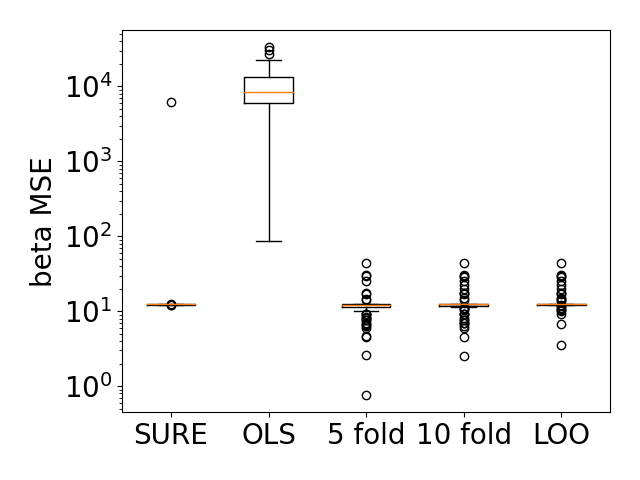
\includegraphics[width=\columnwidth]{../fig/collinear_mse.png}
    \caption{(a) $\|\hbeta - \beta\|_2^2$}
    \label{fig:mse}
\end{subfigure}
\hfill
\centering
\begin{subfigure}[b]{.32\columnwidth} 
    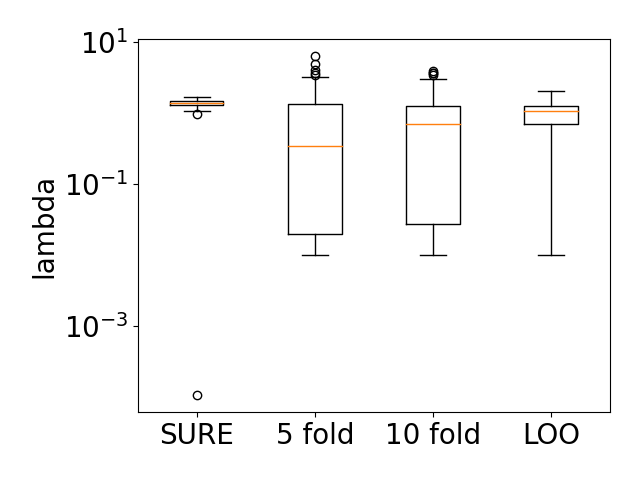
\includegraphics[width=\columnwidth]{../fig/collinear_lambda.png}
    \caption{(b) $\lambda$}
    \label{fig:lambda}
\end{subfigure}
\hfill
\centering
\begin{subfigure}[b]{.32\columnwidth} 
    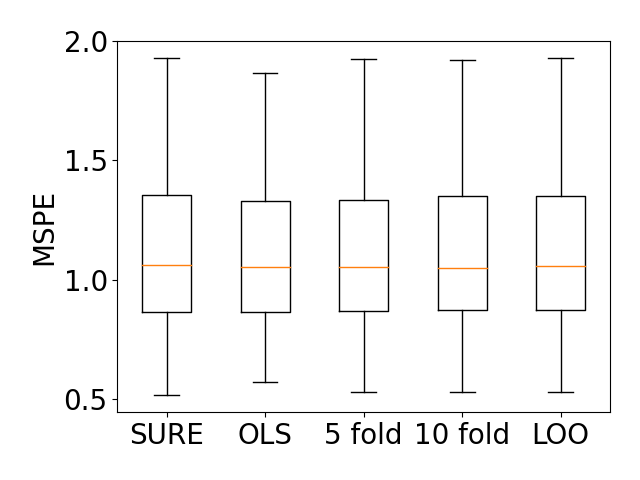
\includegraphics[width=\columnwidth]{../fig/collinear_mspe.png}
    \caption{(c) estimated MSPE}
    \label{fig:mspe}
\end{subfigure}
\caption{Comparison of the $\beta$ MSEs, selected $\lambda$s, and estimated MSPEs using SURE, OLS, 5 fold cross-validation, 10 fold cross-validation, and LOOCV.}
\end{figure}


%\textbf{SURE with Ridge Regression:}
%
%Let $y\sim\distNorm\left( X^T\beta, \sigma^2 \right)$, where $y\in\reals$ and $X\in\reals^{p+1}$, $X$ constant. Then we have $y\sim\distNorm\left( X\beta, \sigma^2I \right)$, where $\biy\in\reals^n$ and $\biX\in\reals^{n\times p}$.
%
%We know that $\hat{\beta}_{\text{ridge}} = \left( X^TX + \lambda I_{p} \right)^{-1}X^Ty$, then 
%\[
%\hat{\mu}_\lambda(\biy) &= \biX\hat{\beta}_{\text{ridge}} = \biX\left( \biX^T\biX + \lambda I_{p+1} \right)^{-1}\biX^T\biy\\
%\hat{\mu}_{\lambda, i}(\biy) &= X_i^T\hat{\beta}_{\text{ridge}} = X_i^T\left( \biX^T\biX + \lambda I_{p+1} \right)^{-1}\biX^T\biy
%\]
%Then
%\[
%\frac{\hat{\mu}_{\lambda, i}(\biy)}{\partial y_i} &= \frac{\partial}{\partial y_i} \left ( X_i^T \left( \biX^T\biX + \lambda I_{p+1} \right)^{-1}\biX^T\biy \right)\\
%&= \frac{\partial}{\partial y_i} F_i \biy \quad\quad (F_i \defas X_i^T\left( \biX^T\biX + \lambda I_{p+1} \right)^{-1}\biX^T \in \reals^{n})\\
%&= F_{i,i}\\
%&= \left( X_i^T\left( \biX^T\biX + \lambda I_{p+1} \right)^{-1}\biX^T \right)_i.
%\]
%We can now write
%\[
%\hat{R} &= -n\sigma^2 + \| \biy - \hat{\mu}_\lambda(\biy) \|_2^2 + 2\sigma^2 \sum_{i=1}^n \left( X_i^T\left( \biX^T\biX + \lambda I_{p+1} \right)^{-1}\biX^T \right)_i\\
%&= -n\sigma^2 + \| \biy - \hat{\mu}_\lambda(\biy) \|_2^2 + 2\sigma^2 \tr\left( \biX\left( \biX^T\biX + \lambda I_{p+1} \right)^{-1}\biX^T \right)\\
%&= -n\sigma^2 + \| \biy - \hat{\mu}_\lambda(\biy) \|_2^2 + 2\sigma^2 \tr\left( \biX^T\biX\left( \biX^T\biX + \lambda I_{p+1} \right)^{-1} \right)\\
%&= -n\sigma^2 + \| \biy - \hat{\mu}_\lambda(\biy) \|_2^2 + 2\sigma^2 \tr\left( H\left( H + \lambda I_{p+1} \right)^{-1} \right),
%\]
%where the last line is by defining $H\defas\biX^T\biX$. We can optimize $\lambda$ over $\hat{R}$ using autodiff (log-transform $\lambda$ so that it is nonnegative). 